\documentclass[10pt,letterpaper]{article} 
\usepackage[margin=1in]{geometry}
\usepackage[utf8]{inputenc}
\usepackage[spanish,english]{babel}

\usepackage{amsmath}
\usepackage{amsfonts}
\usepackage{amssymb}
\usepackage{physics}

\usepackage{graphicx}\graphicspath{{../figs/}}

\usepackage[dvipsnames]{xcolor}

\usepackage{float}

\newcommand{\eref}[1]{eq.~(\ref{#1})} 
\newcommand{\sref}[1]{sec.~\ref{#1}}
\newcommand{\fref}[1]{Fig.~\ref{#1}}
\newcommand{\tref}[1]{table~\ref{#1}}
\newcommand{\Eref}[1]{Eq.~(\ref{#1})} 
\newcommand{\Sref}[1]{Sec.~\ref{#1}}
\newcommand{\Fref}[1]{Fig.~\ref{#1}}  
\newcommand{\Tref}[1]{Table~\ref{#1}}

\usepackage{hyperref}
\hypersetup{
colorlinks=true,
linkcolor=blue,
filecolor=blue,      
citecolor=blue,
urlcolor=blue,
pdftitle={Notes quantum chaos meets quantum channels},
pdfauthor=author={Jose Alfredo de Leon},
}

\usepackage{tikz}

%number lines, show labels, and comments{
\usepackage[mathlines]{lineno}  \linenumbers \setlength\linenumbersep{5pt}
\usepackage[inline]{showlabels,rotating}
\renewcommand{\showlabelrefline}{\hrule width 0pt height 3ex depth 0pt}
\renewcommand{\showlabelfont}{\small\slshape\color{red!70}}
\usepackage[draft,inline,nomargin]{fixme} \fxsetup{theme=color}
\definecolor{jacolor}{RGB}{200,40,0} \FXRegisterAuthor{ja}{aja}{\color{jacolor}JA}
\FXRegisterAuthor{cp}{acp}{\color{blue}CP}
%}

\decimalpoint

\renewcommand{\labelenumii}{\arabic{enumi}.\arabic{enumii}}
\renewcommand{\labelenumiii}{\arabic{enumi}.\arabic{enumii}.\arabic{enumiii}}
\renewcommand{\labelenumiv}{\arabic{enumi}.\arabic{enumii}.\arabic{enumiii}.\arabic{enumiv}}

%comandos para este Tex{
\usepackage{bbm}\newcommand{\one}{\mathbbm{1}}
\newcommand{\mcE}{\mathcal E}
\newcommand{\mcP}{\mathcal P}
\newcommand{\mcD}{\mathcal D}
\newcommand{\mcH}{\mathcal H}
\newcommand{\jami}{Jamiołkowski}
%}

%title, author, date{
\title{Quantum chaos meets quantum channels}
\author{}
\date{\today}
%}

\begin{document}
\maketitle

%\section{Ideas}
%The evolution of the chaometer qubit can be understood as a quantum channel:
%\begin{align}
%\rho_1(t) = 
%\mcE[\rho_1(0)] = 
%\Tr_E\qty(e^{-iHt} \rho_1(0)\otimes \rho_E(0) e^{-iHt}),
%\end{align}
%where $\rho_1(0) \otimes \rho_E(0) = \dyad{\psi(0)}$, 
%with $\ket{\psi(0)}$ is a $L$-qubit random product state; and $H$ the spin chain 
%Hamiltonian.
%
%The quantum channel $\mcE$ can be written in its Kraus form:
%\begin{align}
%\mcE(\rho_1) = 
%\sum_{i=1}^{r\leq 4} K_i \rho_1 K_j^\dagger,
%\end{align}
%with $r$ is the Kraus rank of $\mcE$.
%
%The purity $\mcP$ of the chaometer now reads:
%\begin{align}
%\mcP [\mcE(\rho_1)] &=
%\Tr \big\{\qty[\mcE(\rho_1)]^2 \big\}\\
%&= \sum_{i,j=1}^{r\leq 4}
%\Tr \qty( K_i \rho K_i^\dagger K_j \rho K_j^\dagger) \\
%&= \sum_{i,j}^{r\leq 4}
%\Tr \qty( K_j^\dagger K_i \rho K_i^\dagger K_j \rho).
%\end{align}
%My guess is that the chaotic information of the system has to be 
%encoded in operators $K_i^\dagger K_j$. To further explore this idea 
%I will examine the relationship $\mcP [\mcE(\rho_1)]  = 1 - \eta $.
%
%Integrable:
%\begin{align}
%\mcP [\mcE(\rho_1)] = 
%\min \qty[
%\frac{1}{N} \sum_{i=1}^N 
%\qty(\frac{1}{T}\int_0^T 
%\Tr [\rho_i^2(t)] dt
%)
%] \approx 1
%\end{align}
%
%Chaotic:
%\begin{align}
%\mcP [\mcE(\rho_1)] = 
%\max \qty[
%\frac{1}{N} \sum_{i=1}^N 
%\qty(\frac{1}{T}\int_0^T 
%\Tr [\rho_i^2(t)] dt
%)
%] \approx \frac{1}{2}
%\end{align}

\section{Model}
The spin chain we are interested in studying first is that studied by 
Mirkin and Wisniacki in Ref.~\cite{mirkin2021quantum}:
\begin{equation}\label{eq:H:wisniacki:ising:chain}
H = 
\sum_{i=1}^{L}
\qty(
h_x \sigma_i^x +
h_z \sigma_i^z
) -
\sum_{i=1}^{L-1}
J_z \sigma_{i}^z \sigma_{i+1}^z.
\end{equation}
\section{Mean level spacing ratio}
The level spacing ratio $\tilde r_n$ is defined as:
\begin{equation}\label{eq:level:spacing:ratio}
\tilde r_n= 
\frac{\min(s_n, s_{n-1})}{\max(s_n, s_{n-1})}, 
\end{equation}
where $s_n = E_{n+1} - E_n$. The mean level spacing ratio $\expval{\tilde r_n}$ is 
known to attain the value $\expval{\tilde r_n} \approx 0.5207$ when the 
level spacing distribution $P(s)$ is Wigner-Dyson and
$\expval{\tilde r_n} \approx 0.386$ when it is Poisson.

\begin{figure}
\centering
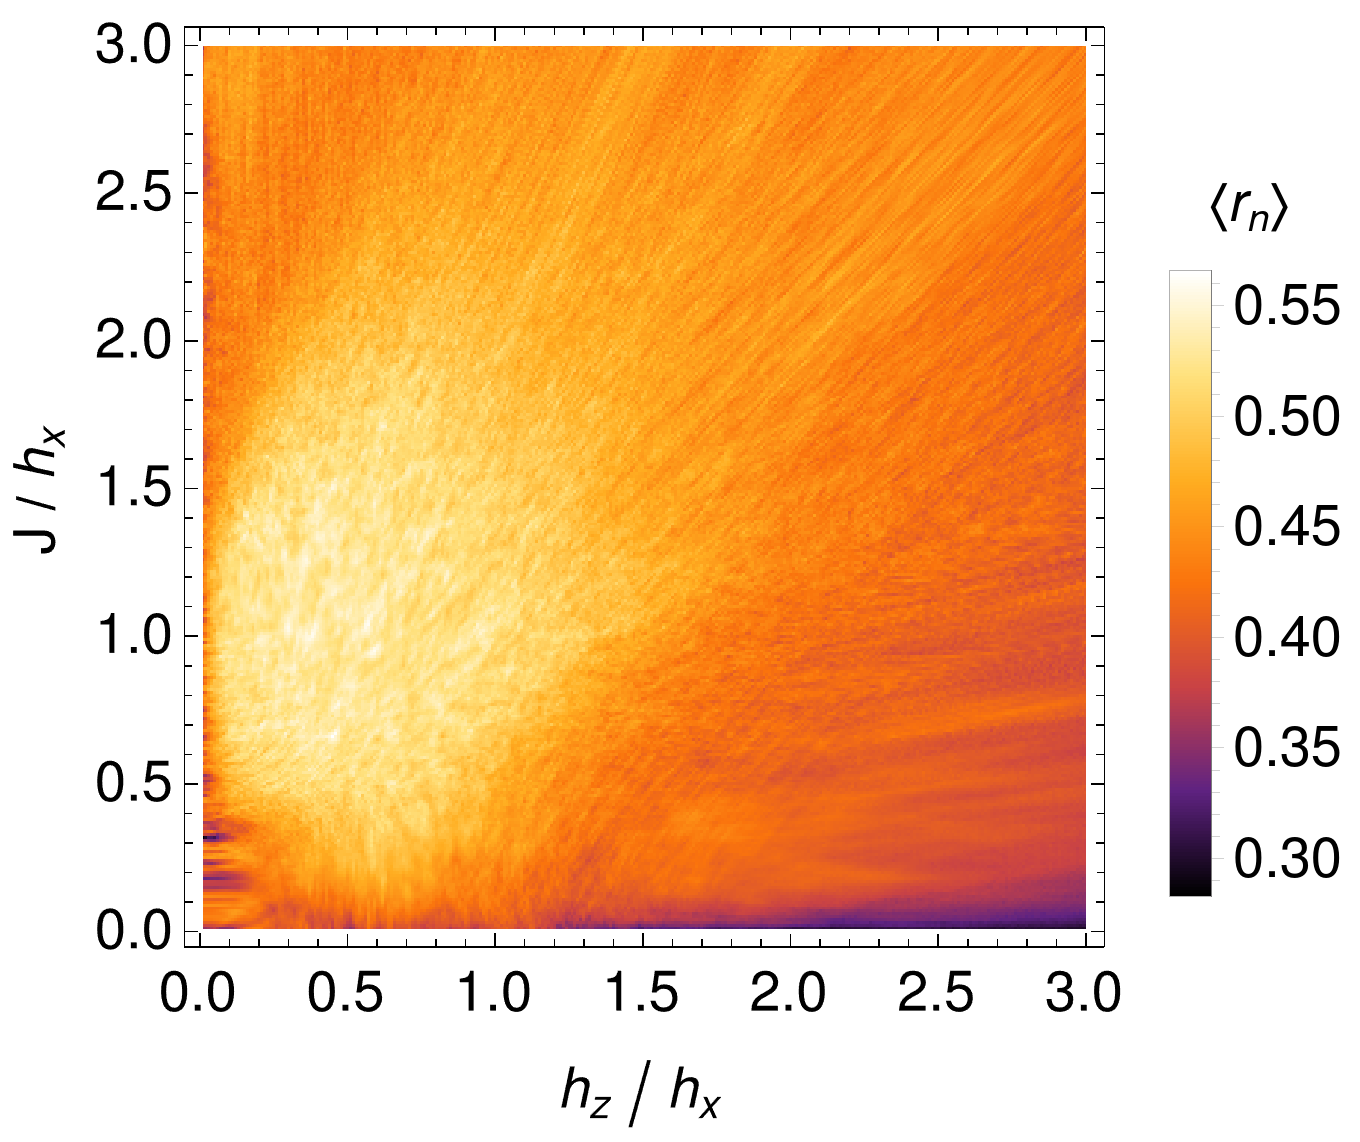
\includegraphics[width=0.7\textwidth]{mean_level_spacing_ratio.png}
\caption{Mean level spacing ratio $\expval{\tilde r_n}$ 
[c.f.~\eref{eq:level:spacing:ratio}] of the Ising chain 
with Hamiltonian \eqref{eq:H:wisniacki:ising:chain} as a function of ratios 
$h_z/h_x$ and $J/h_x$. We assume $J_z=J\, \forall\,k$.}
\label{fig:mean:level:spacing:ratio}
\end{figure}

\section{Spectral form factor}
The spectral form factor $K(t)$ is defined as:
\begin{equation}\label{eq:sff}
K(t) = 
\frac{1}{2^L}
\expval{
\abs{\Tr U(t) }^2
} = 
\frac{1}{2^L}
\expval{
\sum_{i,j} 
e^{i(E_i - E_j) t}
},
\end{equation}
\begin{figure}
\centering
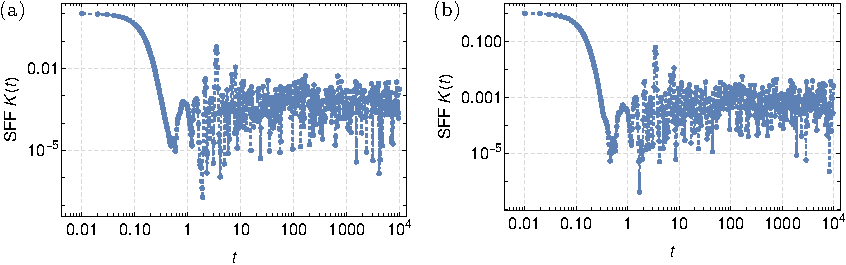
\includegraphics[width=\textwidth]{sff_regular.pdf}
\caption{Spectral form factor (SFF) [c.f.~\eqref{eq:sff}] in regular region: $h_z/h_x=2.5$ and 
$J/h_x=1$. \textbf{(a)} Whole spectrum. \textbf{(b)}~Even-parity subspace 
spectrum.}
\label{fig:sff:regular}
\end{figure}
where $\expval{\cdot}$ denotes the ensemble-average over statistically-similar
systems.

\begin{figure}
\centering
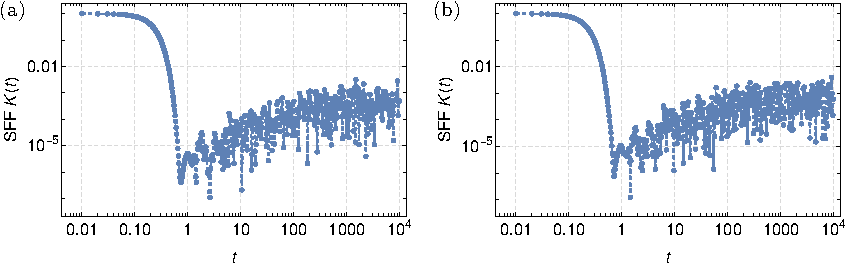
\includegraphics[width=\textwidth]{sff_chaotic.pdf}
\caption{Spectral form factor (SFF) [c.f.~\eqref{eq:sff}] in chaotic region: $h_z/h_x=0.5$ and 
$J/h_x=1$. \textbf{(a)} Whole spectrum. \textbf{(b)}~Even-parity subspace 
spectrum.}
\label{fig:sff:chaotic}
\end{figure}

\section{Chaometer's quantum channel}
The reduced dyanmics of the chaometer is described by the quantum channel: 
\begin{equation}\label{eq:chaometer:channel}
\mcE(\rho) = 
\Tr_E \qty(
e^{-i H t}
\rho \otimes \dyad{\psi_0^{(E)}}
e^{i H t}
),
\end{equation}
where $H$ is that of~\eref{eq:H:wisniacki:ising:chain}, $\ket{\psi_0^{(E)}}$
the initial state of all spins except the chaometer, and $\rho$ the initial 
state of the chaometer. 

The chaometer's quantum channel $\mcE$, in general, is divisible into: 
\begin{enumerate}
\item A unitary operation rotating the Bloch's sphere.
\item A quantum channel that deforms the Bloch's sphere and translates its origin.
\end{enumerate}
Both operations do not commute. 

\janote{Comentar solución de los estados aleatorios.}

\section{Purity of the chaometer}
Averaged purity $\mcP$ is defined in Ref.~\cite{mirkin2021quantum} as:
\begin{equation}\label{eq:avg:purity}
\overline \mcP =
\frac{1}{N}
\sum_{i=1}^{N}
\qty(
\frac{1}{T}
\int_0^T
\Tr \qty[
\rho_i^2(t)
]
)
\end{equation}
where: 
\begin{itemize}
\item $\rho_i(t)$: chaometer's density matrix.
\item $N$: number of different random initial states of the whole chain. 
$N=50$ in Mirkin and Wisniacki~\cite{mirkin2021quantum}.
\item $T$: maximum time. $T=50$ in Mirkin and Wisniacki~\cite{mirkin2021quantum}.
\end{itemize}.

Also, the normalized averaged purity is defined as
\begin{equation}\label{eq:avg:norm:purity}
\overline P_{Norm} = 
\frac{\overline P - \min(\overline P)}{\max(\overline P) - \min(\overline P)},
\end{equation}
where $\max(\overline P)$ and $\min(\overline P)$ are the minimum and maximum
value obtained when sweeping the parameter range ($h_z$ in their case). 

In~\Fref{fig:purity:one:realization} we plot one realization of the dynamics 
of purity of the chaometer. 
We compare in \Fref{fig:mirkin2021:fig2:modified} our results and those 
of Mirkin and Wisniacki~\cite{mirkin2021quantum}.

\section{Purity of Choi-\jami{} matrix}
We investigate the purity of Choi-\jami{} matrix of quantum channel $\mcE(t)$ 
of the chaometer [c.f.~\eref{eq:chaometer:channel}] in \Fref{fig:choi:purity}.

\begin{figure}
\centering
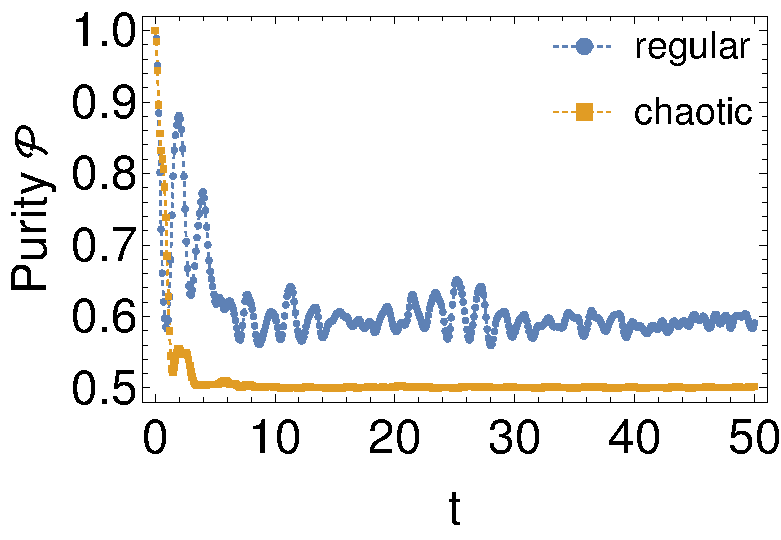
\includegraphics[width=.6\textwidth]{purity_one_realization.pdf}
\caption{Dynamics of chaometer's purity of a single realization 
with the same initial state of the environment of the first chaometer's 
quantum channel of the videos.}
\label{fig:purity:one:realization}
\end{figure}
\begin{figure}
\centering
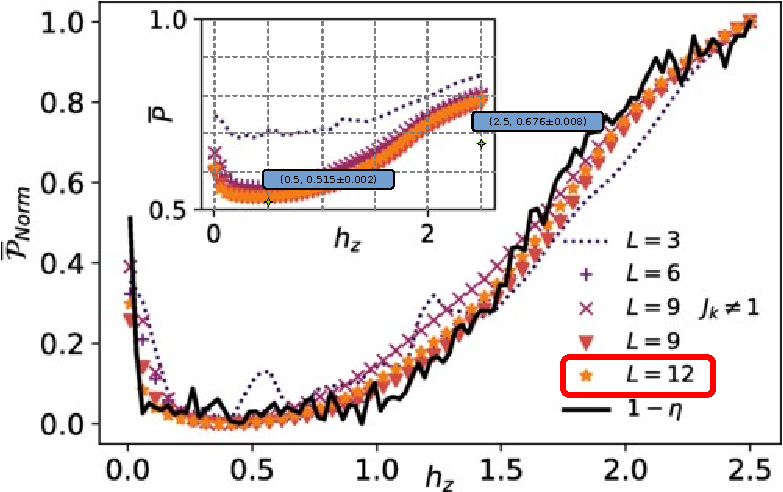
\includegraphics[width=0.9\linewidth]{mirkin2021_fig2_modified.pdf}
\caption{Averaged $\overline P$ and averaged normalized purities 
$\overline P_{Norm}$ [c.f. eqs.~\eqref{eq:avg:purity} and~\eqref{eq:avg:norm:purity}.] for $N=50$ random initial states of 
the chaometer for each quantum channel showed in the videos.
\janote{Tendría más sentido sacar la pureza del canal. Lo pienso}
Taken and modified from Ref.~\cite{mirkin2021quantum}.}
\label{fig:mirkin2021:fig2:modified}
\end{figure}
\begin{figure}
\centering
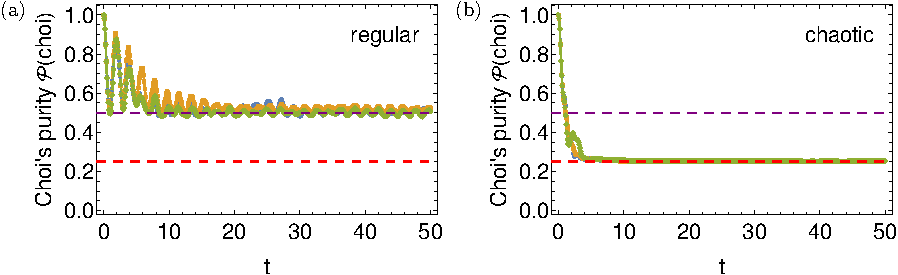
\includegraphics[width=\textwidth]{choi_purity.pdf}
\caption{Purity of Choi-\jami{} matrix in (a) regular ($h_z=2.5$) and (b) chaotic ($h_z=0.5$) for the three random initial states showed in the video.}
\label{fig:choi:purity}
\end{figure}

To compute the Choi-\jami{} matrix $\mcD(t)$ of the chaometer's quantum channel 
in~\eref{eq:chaometer:channel} we use the definition 
$\qty(\mcE \otimes \one) \qty[\dyad{\phi^+}]$, with $\ket{\phi^+}=1/\sqrt{2}\qty(\ket{0,0} + \ket{1,1})$
is the maximally entangled state between two spins, and obtain
\begin{align}\label{eq:choi:chaometer}
\mcD(t) &= 
\frac{1}{2}
\sum_{i,j,p,q}
\bra{j, \psi_{0E}} U^\dagger(t) \qty( \dyad{p}{q}\otimes \one_E ) U(t)
\ket{i, \psi_{0E}} \dyad{q,i}{p,j}.
\end{align}

Let us write $\mcE(\rho)$ in computational basis. From \eref{eq:chaometer:channel}
we write
\begin{align}
%{
\mcE(\rho) &= 
\sum_{k,l} 
e^{-i (E_k - E_l)t}
\bra{E_k}  \qty(\rho \otimes \dyad{\psi_{E}}) \ket{E_l} \Tr_E \qty(\dyad{E_k}{E_l})\\
%}
%{
&= 
\sum_{k,l, p, p', \vec q, \vec q'}
e^{-i (E_k - E_l)t}
\bra{E_k} 
\qty(\rho \otimes \dyad{\psi_{E}}) 
\ket{E_l} 
\Tr_E \qty( \ket{p,\vec q} \braket{p,\vec q}{E_k} 
\braket{E_l}{p', \vec q'} \bra{p', \vec q'}), \\
%}
\intertext{where $\vec q$ and $\vec q'$ are indices of elements of the 
basis of the environment,}
%{
&= 
\sum_{p, p', \vec q}
\bra{p, \vec q}
U(t) \qty(\rho \otimes \dyad{\psi_{E}}) U^\dagger(t)
\ket{p', \vec q}
\dyad{p}{p'} \\
%}
%{
&= \label{eq:chaometer:channel:2}
\sum_{p, p'}
\bra{p}
\Tr_E[U(t) \qty(\rho \otimes \dyad{\psi_{E}}) U^\dagger(t) ]
\ket{p'}
\dyad{p}{p'}.
%}
\end{align}

To compute the Choi-\jami{} matrix $\mcD(t)$ of the chaometer's quantum channel 
in~\eref{eq:chaometer:channel} we use the definition 
$\qty(\mcE \otimes \one) \qty[\dyad{\phi^+}]$, with $\ket{\phi^+}=1/\sqrt{2}\qty(\ket{0,0} + \ket{1,1})$
is the maximally entangled state between two spins, and \eref{eq:chaometer:channel:2} to obtain
\begin{align}
%{
\mcD(t) &=  
\frac{1}{2} 
\sum_{i, j, p, p', \vec q}
\bra{p, \vec q}
U(t) \qty(\dyad{i,\psi_{E}}{j,\psi_{E}}) U^\dagger(t)
\ket{p', \vec q}
\dyad{p,i}{p',j} \\
%}
%{
&= \label{eq:choi:chaometer:computational:basis}
\frac{1}{2}
\sum_{i, j, p, p'}
\bra{j, \psi_{0E}} U^\dagger(t) \qty( \dyad{p'}{p}\otimes \one_E ) U(t)
\ket{i, \psi_{0E}} \dyad{p, i}{p', j},
%}
\end{align}
where we have only reordered the factors and used the resolution of identity over 
$\mcH_E$.

We compute the purity of $\mcD(t)$. From \eref{eq:choi:chaometer} 
it is straightforward to obtain
\begin{align}\label{eq:choi:chaometer:purity:1}
\Tr[\mcD^2(t)]  &= 
\frac{1}{4}
\sum_{i,j,p,q}
\abs{\matrixel{i, \psi_{0E}}
{U^\dagger(t) \big(\dyad{p}{q} \otimes \one_E\big) U(t)}
{j, \psi_{0E}}
}^2.
\end{align}
Moreover, reordering this expression an interesting interpretation of the purity 
of the Choi-\jami{} matrix is revealed. Let us conveniently rewrite
\eref{eq:choi:chaometer:purity:1} as
\begin{align}\label{eq:choi:chaometer:purity:2}
\Tr[\mcD^2(t)]  &= 
\bra{\psi_{0E}}
\Tr_S\{
U^\dagger(t) 
\sum_{p, q} \qty[
\qty(\frac{\dyad{p}{q}}{\sqrt{2}} \otimes \one_E ) 
U(t)
\qty( \frac{\one_S}{2} \otimes \dyad{\psi_{0E}})
U^\dagger(t) 
\qty(\frac{\dyad{q}{p}}{\sqrt{2}} \otimes \one_E ) 
]
U(t)\}
\ket{\psi_{0E}}.
\end{align}
\janote{esta es una especie de echo de Loschmidt!!!}
In other words, the purity of $\mcD(t)$ represents the probability that the 
environment remains in its initial state after the following process: First, the system
and environment are initialized in a product state, with the system in a maximally
mixed state. Next, the combined system evolves. Then, a completely depolarizing
channel is applied to the system. Finally, the system and environment undergo 
reverse evolution.

The Loschmidt echo is defined as
\begin{equation}\label{eq:loschmidt:echo}
M(t) = 
\abs{\expval{e^{-i H_2 t/\hbar}e^{-i H_1 t/\hbar}}{\psi_0}}^2
\end{equation}

\section{Non complete positiveness of $\Lambda(t, s)$}
Any quantum channel $\mcE(t)$ can composed as 
\begin{equation}\label{eq:Lambda}
\mcE(t) = 
\Lambda(t,s) \circ \mcE(s, 0),
\end{equation}
nonetheless, $\Lambda(t,s)$ is not in general completely positive. A way to 
quantify how far is $\Lambda(t,s)$ from being completely positive is through 
$\tilde \lambda$:
\begin{equation}\label{eq:lambda:tilde}
\tilde \lambda = 
\abs{\min(0, \lambda_{\text{smallest}})},
\end{equation}
where $\lambda_{\text{smallest}}$ is the smallest eigenvalue of 
$\Lambda^R(t,s)/2$. We have added the factor $1/2$ just so 
$\Tr[\Lambda^R(t,s)/2]~=~1$.

Let us fix $s=0.1$ and investigate the complete positiviness of 
$\Lambda(t, s)$, see \Fref{fig:lambda:tilde:Choi-\jami{}}.

\begin{figure}
\centering
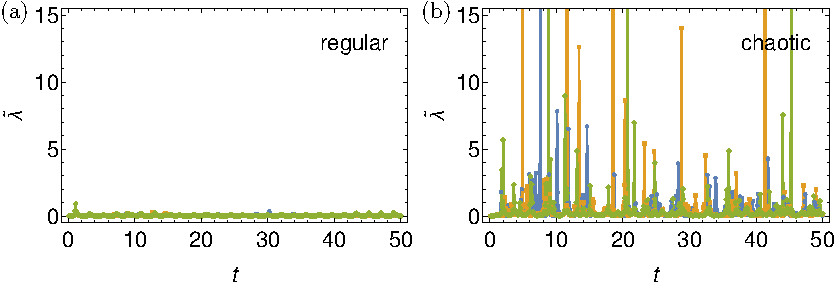
\includegraphics[width=\textwidth]{lambda_tilde_choi.pdf}
\caption{Most negative eigenvalue $\tilde \lambda$ of map $\Lambda(t,s)/2$, 
with $s=0.1$ [c.f. eqs.~\eqref{eq:Lambda}~and~\eqref{eq:lambda:tilde}].}
\label{fig:lambda:tilde:Choi-\jami{}}
\end{figure}

\begin{figure}
\centering
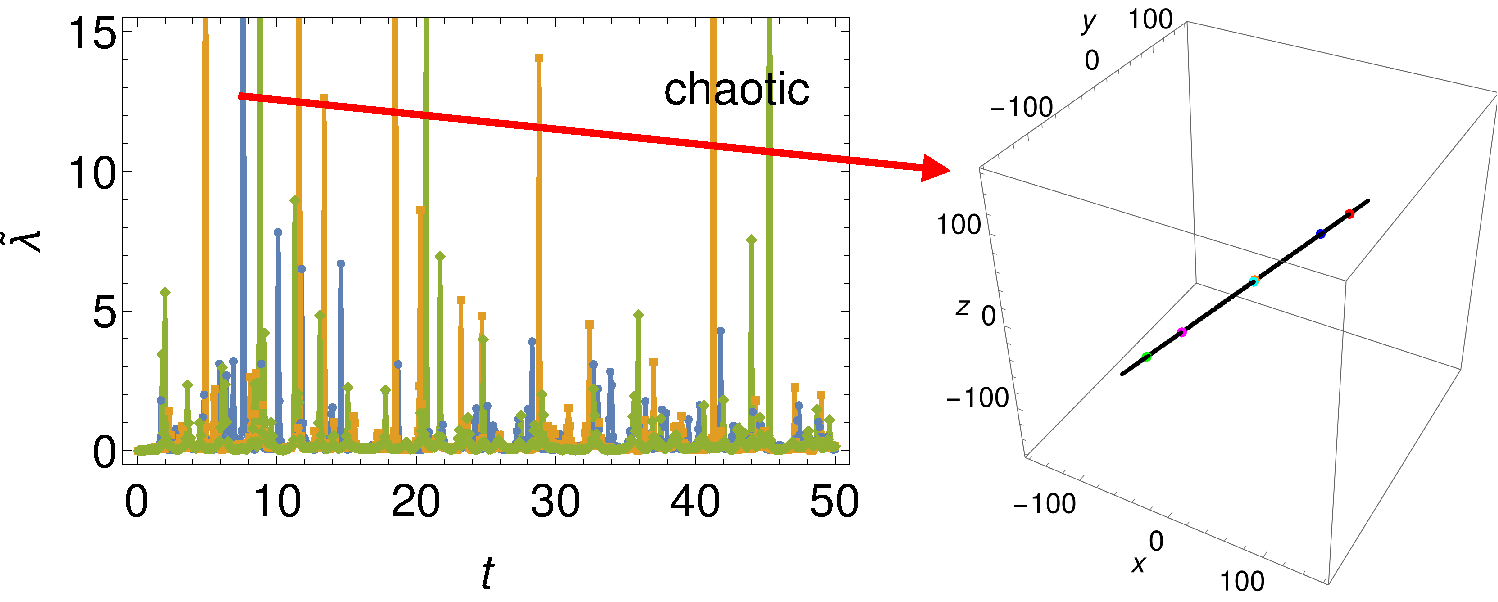
\includegraphics[width=\textwidth]{burst.pdf}
\caption{Burst of the Bloch sphere at $t=0.5$ s.}
\label{fig:burst}
\end{figure}

\section{Purity of Choi-\jami{} matrix of a U from COE}

\begin{figure}
\centering
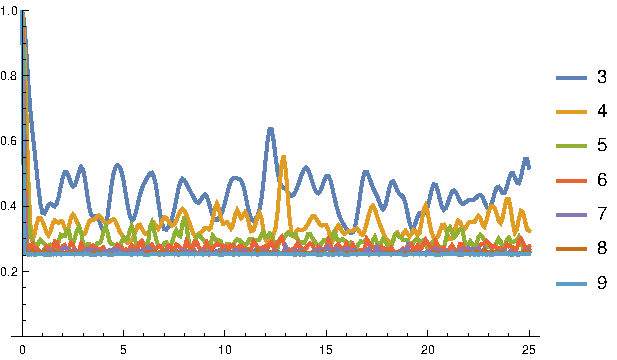
\includegraphics[width=0.7\textwidth]{choi_purity_goe_L_3_to_9.pdf}
\caption{
\janote{La pureza de la matriz de Choi de una matriz U de COE se comporta así
variando el número de espines $L$ desde 3 hasta 9. Parece que para $L$ muy grande
el límite asintótico tiende a 0.25, Se podrá probar analíticamente? }}
\end{figure}
\begin{figure}
\centering
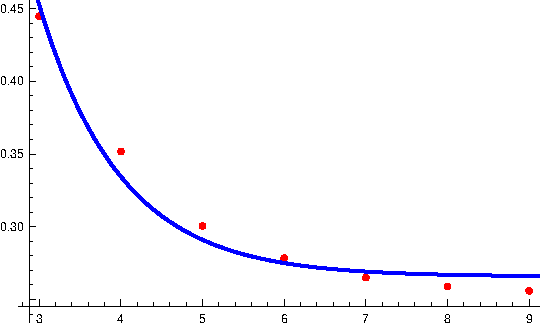
\includegraphics[width=0.7\linewidth]{choi_purity_goe_asymptotic_vs_L.pdf}
\caption{
\janote{$\Tr[\mcD^2_\infty]$ vs $L$. Creo que se podría conseguir un mejor ajusto
teniendo estadística para cada punto.}
}
\end{figure}

%{
% !TEX root = main.tex
\section{Charles}
% !TEX root = main.tex
\section{Miguel}
% !TEX root = main.tex
\section{Viko}
%}


%bibliography{{{
\bibliographystyle{unsrt}
\bibliography{references.bib}
%}}}

\end{document}